\documentclass{article}
\usepackage{microtype}
\usepackage{graphicx}
\usepackage{booktabs}
\usepackage{hyperref}
\usepackage{amsmath,amssymb,amsthm}
\usepackage{tikz}
\usetikzlibrary{arrows.meta,positioning,fit}
\usepackage[accepted]{icml2025}
\newtheorem{theorem}{Theorem}
\icmltitlerunning{Scheduling LLM Agents under KV-Cache Pressure (Midterm Report)}

\begin{document}
\twocolumn[
\icmltitle{Provably Good Scheduling of LLM Agents under KV-Cache Pressure}
\begin{icmlauthorlist}
\icmlauthor{[Author names]}{h}
\end{icmlauthorlist}
\icmlaffiliation{h}{Harvard University, CS 243 (Fall 2026). Midterm report}
\icmlcorrespondingauthor{[Author]}{[email]}
\icmlkeywords{LLM serving, agents, scheduling, KV cache, approximation algorithms}
\vskip 0.3in
]
\printAffiliationsAndNotice{}

\begin{abstract}
LLM agents alternate between model calls and tool calls of unpredictable length, and many agents share one GPU.
When KV-cache memory is scarce, the serving engine's choice of \emph{which agent to serve next} decides how long
every task takes, yet today's engines schedule individual requests first-come-first-served and agent-aware
systems use heuristics without guarantees. We model agent serving as stochastic scheduling of task graphs with
random tool delays on a batched engine with bounded KV memory, and derive a \emph{task index} $Z'$ that ranks
whole agent tasks by their total cost to the GPU, including the memory they occupy and the recomputation that
tool waits cause. We prove that scheduling by this index is within a constant factor of the optimal
non-anticipatory policy (factor 2, tight, without memory limits; about 5--7 with KV memory at our measured A40
parameters); two independent verification passes checked every proof. We implemented the index on vLLM as a
drop-in scheduler plug-in and client layer. On four A40 GPUs serving Qwen3-8B to multi-hop question-answering
agents under KV pressure, it cuts the \textbf{median task completion time by 37\%} (42\,s to 27\,s) and the mean
by 19\% relative to vLLM, improves \textbf{every one of seven workloads}, and beats a Continuum-style agent
scheduler by 47\% on the median.
\end{abstract}

\section{Problem}
\label{sec:problem}
An LLM agent task is a small program: it calls the model, calls tools (search, code, APIs) whose latency is long
and random compared with a model step, often several in parallel~\cite{kim2024llmcompiler}, and calls the model
again on the results~\cite{yao2023react}. A serving engine such as vLLM~\cite{kwon2023vllm} sees only the
individual model calls. It admits them first-come-first-served (FCFS), and while an agent waits for a tool, its
KV cache either occupies scarce GPU memory or is evicted and later recomputed.

\textbf{Why scheduling matters here.} Under memory pressure only a few agents fit on the GPU at once, so the
order in which tasks are served dominates latency. Per-request FCFS is a poor order for agents: a task's latency
is set by its \emph{last} model call, and a long task that arrives first blocks many short tasks behind it, each
of which also holds memory across its tool waits.

\textbf{Why it is new.} Agent-aware systems schedule at the program level, with heuristics:
Continuum~\cite{li2025continuum} pins an agent's KV cache for a time-to-live during tool calls and serves
programs FCFS, Autellix~\cite{luo2025autellix} ranks programs by least attained service, and
LAMPS~\cite{shahout2024lamps} ranks requests by memory consumption over time and chooses whether to keep or
discard memory during API calls. None comes with a performance guarantee. On the theory side, recent online
algorithms for KV-constrained LLM scheduling~\cite{jaillet2025online} treat single requests, with no tool calls,
task graphs or random durations, and classical stochastic scheduling~\cite{mohring1999approximation,
skutella2005stochastic} has no batching, KV memory or tool delays. To our knowledge, ours is the first
scheduling policy for agent serving with a provable approximation guarantee.

\textbf{Challenges.} (1) Tool delays and output lengths are random and unknown when decisions are made. (2) GPU
time and KV memory are coupled: evicting a waiting agent frees memory but costs recomputation, and a batched step
slows down as more sequences join it. (3) Latency belongs to whole tasks, while the engine schedules individual
calls. (4) A guarantee must survive contact with a real engine: vLLM's admission, preemption and caching rules.

\section{Design}
\label{sec:design}

\textbf{Model.} A task $J$ arrives at time $r_J$ with weight $w_J$ and is a directed acyclic graph of LLM
nodes; tool calls are random delays on the edges. Node $y$ has a new prompt of $q_y$ tokens, a context of
$\rho_y$ tokens carried from earlier calls, and at most $X_y$ output tokens. The engine runs batched steps of
duration $a + cB + \alpha P$ for $B$ decoding sequences and $P$ prefill tokens, and the KV cache holds at most
$M$ tokens. On our A40 with Qwen3-8B we measured $a = 27.8$\,ms, $c = 0.54$\,ms and $\alpha = 0.11$\,ms per
token. The objective is the expected weighted sum of task completion times, $\mathbb{E}[\sum_J w_J C_J]$.

\textbf{The task index.} Each task gets one number when it arrives,
\begin{equation}
Z'_J = \sum_{y \in J} \Big[\alpha(q_y+\rho_y) + cX_y + \alpha(\ell_y + L_{\max}) + \frac{a X_y \ell_y}{M'}\Big],
\label{eq:z}
\end{equation}
where $\ell_y = \rho_y + q_y + X_y$ is the node's peak KV footprint, $L_{\max}$ the largest footprint and $M'$
the usable memory. The four terms are the node's prefill work (including recomputing evicted context after a
tool wait), its decode work, a charge for the work it may displace when it is admitted, and its share of the
memory-time area. Tasks are served in increasing order of $Z'_J/w_J$, a memory-aware generalization of Smith's
rule~\cite{smith1956various}. The index is fixed for the task's lifetime, so a task never loses its place to
newer arrivals of the same size.

\textbf{Guarantees.} Let $\mathrm{OPT}$ be the best non-anticipatory policy (it knows distributions, not the
future).
\begin{theorem}[no memory limit]
For task graphs with known node sizes and arbitrary random tool delays, on $m$ parallel servers, the online
preemptive policy that runs tasks in order of $w_J/W_J$ (total work $W_J$) satisfies
$\mathbb{E}[\sum w_J C_J] \le 2\,\mathrm{OPT}$, and the factor 2 is tight.
\end{theorem}
\begin{theorem}[batched engine with KV memory]
In the engine model above, the policy that ranks tasks by $w_J/Z'_J$, admits the longest priority prefix of
requests whose reservations fit in memory, and evicts KV during tool waits, satisfies
$\mathbb{E}[\sum w_J C_J] \le c\cdot\mathrm{OPT}$ with $3\times$ engine speed and $M + L_{\max}$ memory, where
$c$ depends only on the ratio of recomputation to useful work; $c \approx 5$--$7$ at our measured parameters for
$M$ between 32k and 128k tokens.
\end{theorem}
Theorem~1 extends Megow and Schulz~\cite{megow2004online} to task graphs with random tool delays: delays enter
only through the critical path. Theorem~2 is new; its key step charges every preemption to the arrival that
caused it. We also proved a 2-approximation for chain tasks with random sizes (a Gittins-index variant), that
keeping KV across tool waits never breaks Theorem~2 if kept KV is evicted first, and that the best keep/evict
time-to-live for a known delay distribution is within $e/(e-1)$ of clairvoyant. Two independent verification
passes checked every proof; each inequality is also checked exactly on small instances, and the algebra with
the Z3 solver (7{,}772 automated tests).

\begin{figure}[t]
\centering
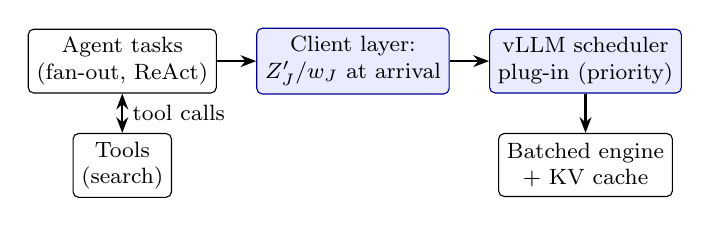
\begin{tikzpicture}[font=\footnotesize, node distance=4mm and 5mm,
  box/.style={draw, rounded corners=2pt, align=center, inner sep=3pt, minimum height=8mm},
  ours/.style={box, fill=blue!8, draw=blue!60!black},
  arr/.style={-{Stealth[length=2mm]}, thick}]
\node[box] (agents) {Agent tasks\\(fan-out, ReAct)};
\node[ours, right=of agents] (client) {Client layer:\\$Z'_J/w_J$ at arrival};
\node[ours, right=of client] (sched) {vLLM scheduler\\plug-in (priority)};
\node[box, below=5mm of agents] (tools) {Tools\\(search)};
\node[box, below=5mm of sched] (engine) {Batched engine\\+ KV cache};
\draw[arr] (agents) -- (client);
\draw[arr] (client) -- (sched);
\draw[arr] (sched) -- (engine);
\draw[arr, {Stealth[length=2mm]}-{Stealth[length=2mm]}] (agents) -- node[right]{tool calls} (tools);
\end{tikzpicture}
\caption{Implementation. The client layer computes each task's index once and attaches it as the priority of
every model call the task makes; a scheduler plug-in loaded with \texttt{--scheduler-cls} applies it inside
vLLM. Shaded boxes are ours.}
\label{fig:design}
\end{figure}

\textbf{Implementation (Figure~\ref{fig:design}).} The system needs no fork of vLLM. A client layer (130
lines) computes $Z'_J$ from token-count estimates when a task arrives and sends it as the priority of each of the
task's model calls. A scheduler subclass (360 lines), loaded through vLLM~0.32's \texttt{--scheduler-cls}
option, adds the engine rules the theory uses: priority-prefix admission with preemption, a single prefill per
step, a low-priority class for speculative prefills, a soft time-to-live for KV kept during tool waits, and
protection of cached prefixes that queued requests need. All rules are switches, so baselines run through the
same code. In this report \emph{Ours} is the index on top of vLLM's priority scheduler; the engine rules are
evaluated as ablations (Section~\ref{sec:plan}).

\section{Initial Evaluation}
\label{sec:eval}

\textbf{Setup.} Four NVIDIA A40 GPUs (48\,GB), one vLLM~0.32 server per GPU, Qwen3-8B~\cite{qwen3} in bf16.
Agents answer multi-hop HotpotQA questions~\cite{yang2018hotpotqa} with a search tool over a pool of
HotpotQA paragraphs, in two shapes: \emph{fan-out} (plan, then 2, 4 or 8 parallel searches, then answer) and
\emph{ReAct} (2, 4 or 6 search-and-reason turns). Search results are up to 1{,}000 tokens; tool delays are
uniform on 0.5--4\,s with probability 0.7 and on 4--12\,s otherwise. Tasks arrive as a Poisson process at 1 per
second for 90\,s (about 93 tasks per run). To emulate the memory pressure of a busier multi-tenant server, we
cap the KV cache at 16k tokens (full capacity is 167k). Each \emph{seed} fixes the arrival times, task mix and
tool delays, and every scheduler sees exactly the same seed, so comparisons are paired task by task. We report
task completion time, from arrival to final answer.

\textbf{Baselines.} \emph{vLLM}: stock scheduler, requests FCFS. \emph{Continuum-like}: our reimplementation of
Continuum's policy~\cite{li2025continuum}: KV pinned during tool calls with a time-to-live, programs served
FCFS, pinned programs first. \emph{Autellix-like}: Autellix's program-level least-attained-service
ranking~\cite{luo2025autellix}.

\begin{figure*}[t]
\centering
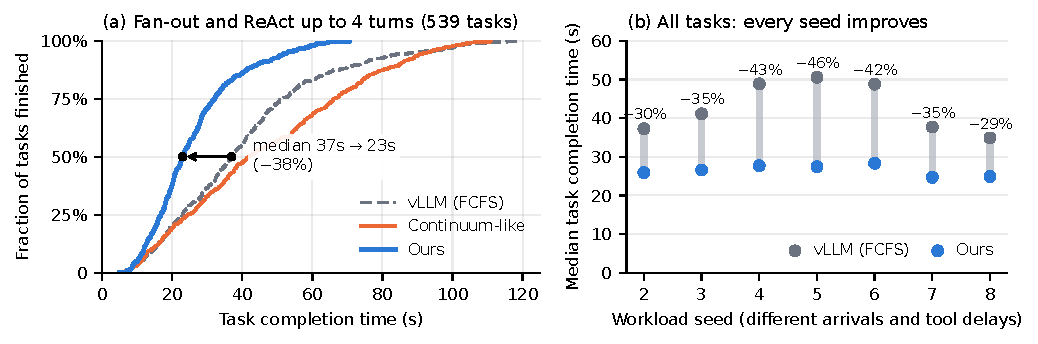
\includegraphics[width=0.92\textwidth]{figs/headline.pdf}
\vspace{-2mm}
\caption{Task completion times at 16k tokens of KV memory. (a) Distribution over all 653 tasks of seven
workloads: with our index, 75\% of tasks finish within 45\,s, versus 68\,s with vLLM. (b) Median per workload:
our index improves every seed, by 29--46\% (mean: 11--24\%).}
\label{fig:headline}
\end{figure*}

\begin{table}[t]
\caption{All tasks at 16k tokens of KV memory, seven seeds (653 paired tasks). ``Faster'': share of tasks that
finish earlier than under vLLM.}
\label{tab:main}
\centering
\small
\begin{tabular}{lccc}
\toprule
Scheduler & Mean (s) & Median (s) & Faster \\
\midrule
vLLM (FCFS) & 50.3 & 42.0 & -- \\
Continuum-like & 52.1 & 50.7 & 48\% \\
Autellix-like$^{*}$ & 65.9 & 47.3 & 49\% \\
\textbf{Ours ($Z'$ index)} & \textbf{40.6} & \textbf{26.7} & \textbf{79\%} \\
\bottomrule
\end{tabular}

\vspace{1mm}
{\footnotesize $^{*}$Run with our preemptive admission rule.}
\end{table}

\textbf{Results.} Figure~\ref{fig:headline} and Table~\ref{tab:main} show the main result. Under memory
pressure, scheduling by the task index cuts the median completion time from 42\,s to 27\,s ($-37\%$, 95\% CI
31--43\%) and the mean from 50.3\,s to 40.6\,s ($-19\%$, CI 15--23\%), and 79\% of tasks finish earlier. The
improvement holds on every one of the seven workloads (Figure~\ref{fig:headline}b). Against the
Continuum-like scheduler, the median drops by 47\% (CI 36--54\%) and the mean by 22\%. Confidence intervals
come from a two-level bootstrap that resamples whole workloads and then tasks, so they include run-to-run
variation.

The gain is broad across task types. For fan-out tasks the mean falls by 34\% (32.9\,s to 21.6\,s), and for
two-search fan-outs and two-turn ReAct agents by 41\% and 45\%. Fan-out tasks finish twice as fast as under the
Continuum-like scheduler (21.6\,s versus 42.8\,s on average).

\begin{figure}[t]
\centering
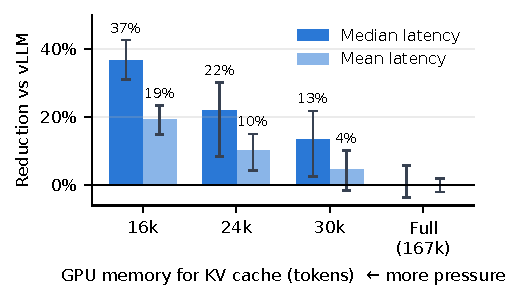
\includegraphics[width=\columnwidth]{figs/memory.pdf}
\vspace{-5mm}
\caption{Latency reduction of our index over vLLM as KV memory grows (95\% CIs). The tighter the memory, the
larger the gain; with ample memory scheduling order barely matters and the index costs nothing.}
\label{fig:memory}
\end{figure}

\textbf{When does it help?} Figure~\ref{fig:memory} repeats the experiment with more KV memory (three seeds
each at 24k, 30k and full memory). The benefit grows with memory pressure: the median falls by 22\% at 24k and
13\% at 30k, and at full memory the index matches vLLM. This matches the model: the index
matters when memory limits how many agents run at once, which is the regime of busy multi-tenant deployments,
long contexts and large tool outputs.

\section{Remaining Challenges and Plan}
\label{sec:plan}
\textbf{1. Isolate what the index contributes.} With equal weights, $Z'$ ranks tasks by estimated cost. We will
compare it on equal footing with simpler rankings: smallest estimated task first, Autellix's ranking on stock
admission (our Autellix-like run above used our preemptive admission), and a LAMPS-style memory-area
ranking~\cite{shahout2024lamps}. This decides whether the memory and recomputation terms of
Eq.~\eqref{eq:z} matter in practice.

\textbf{2. Protect the longest tasks.} Ranking by cost makes the largest tasks wait: six-turn ReAct agents
finish 14\% later than under vLLM, and the 90th percentile does not improve (106\,s versus 101\,s). We will add aging (the index
improves while a task waits) and check that the guarantee survives it.

\textbf{3. Close the theory--practice gap on admission.} Theorem~2 needs admission in strict priority order with
preemption. In our ablations this rule costs latency on long tasks, because preempted requests recompute their
context; likewise, keeping KV across tool waits added no measurable gain on top of the index at this scale. We
will look for an admission rule without preemption that keeps a constant-factor guarantee, and test KV retention
with longer contexts and tool outputs, where recomputation is expensive.

\textbf{4. Broaden the evaluation.} More arrival rates and memory sizes, a larger model, and measuring how close
each run comes to the theory's lower bound on $\mathrm{OPT}$, which tests whether the proven constant is pessimistic.

\textbf{Timeline.} Items 1 and 2 by the presentation (12/1); items 3 and 4 and the final report by 12/16. Our
earlier study of KV preloading of tool results, which motivated the engine rules, is complete and serves as a
fallback.

\bibliography{refs}
\bibliographystyle{icml2025}

\end{document}
